\chapter{Introduction}
During the course of my PhD investigations, I have primarily focussed on the phenomenology of a model of
interacting stochastic particle motion through lattices, called the \textbf{Sticky Particle Model} (SPM). In
this chapter we motivate and define this model, and then explore some of its more basic properties and
association with existing models in the literature.

\section{Derivation and Motivation of the Sticky Particle Model}
\subsection{The Motion of Small Atoms in Crystal Lattices}
Consider a material composed of a regular crystalline lattice of a single type of atom. Most pure metals
are like this in at least part of their solid phase. For example, under standard conditions Iron is such
a material, and will typically try and assume a body-centred cubic (bcc) structure~\cite{Villars2016}, whilst Titanium tends to
form a hexagonal close-packed (hcp) structure~\cite{Patterson1925}.

It is often possible for impurities to enter such a crystalline material.  In many
situations, these invading atoms are smaller than those of
which the bulk material is composed~\cite{DealGrove1965, tegner2015}. Such small impurity atoms can reside in the interstitial spaces between 
the crystal atoms, and they will sometimes move between adjacent interstitial sites. This motion is
stochastic in nature, as it depends upon the impurity possessing sufficient momentum to squeeze between
the lattice atoms and travel to the next site, or those atoms perhaps moving apart a little to allow easier
passage; both of these processes are dominated by thermal effects at finite temperature, and the end result
is that the impurity atom will tend to hop from one interstitial site into an
adjacent one essentially at random, with some rate $\tau_0 ^{-1} \mathrm{s}^{-1}$.
Such rates can be determined either by actual experiments (e.g. tracer diffusion
~\cite{Lamb1946, Wersin2004}) or by theoretical means
(e.g. molecular dynamics~\cite{Zhang1994, keffer2001}).

A single such impurity atom will obviously perform some kind of random walk though the system, and those kinds
of mathematics have been treated previously. In this work, we really want to consider what effects these
particles have upon each other as they hop around, via their interactions; thus, we think it best that we
perform simplifications in order to strip out any nonessential details, so that we can focus on effects 
caused by interaction. Therefore we won't be calculating any
transition rates for real systems.

\subsection{Reduction to 1D, Simplifications, and Model Definition}
\label{sec:modelDefn}
A crystal in physical reality is typically $3$-dimensional 
\footnote{or possibly $2$-dimensional, but those
are odd cases~\cite{allen2009}}.
However, a lot of the time these $3$D crystals can be quite anisotropic. For example, in
an hcp crystal lattice, the complementary lattice of octahedral interstitial sites form a simple hexagonal
structure, consisting of stacked planes of hexagonal lattices~\cite{Li2018}. Thus, it is not too difficult to envision
a situation in which the hopping rate is much faster between planes than within them, or vice-versa. In the
first situation, if there were sufficient discrepancy between the interplanar and intraplanar hopping rates
we would essentially have a series of decoupled $1$ or $2$-dimensional systems.

We should also remember that it is often much easier to use analytical techniques in one dimension than
in higher dimensions, and that the performance of numerical techniques often scales unfavourably 
with dimension. Therefore, we have chosen to concentrate on the $1$D case for the time being, and will then
return to the issue of higher dimensions in Sec.~\ref{sec:highDimSPM}.

A particle hopping back and forth in $1$D would experience a periodic potential energy arising from the 
background lattice, perhaps like the one displayed in Fig.~\ref{fig:periodicPot}.
\begin{figure} \caption[An impression of the kind of background potential experienced by a particle moving
against a periodic lattice in $1$D.]{A simple example of the kind of background potential experienced by a 
particle moving against a periodic lattice in $1$D. Here the potential is represented by $f(x)$, where $a$
is the lattice spacing.} 
\label{fig:periodicPot}
\begin{center}
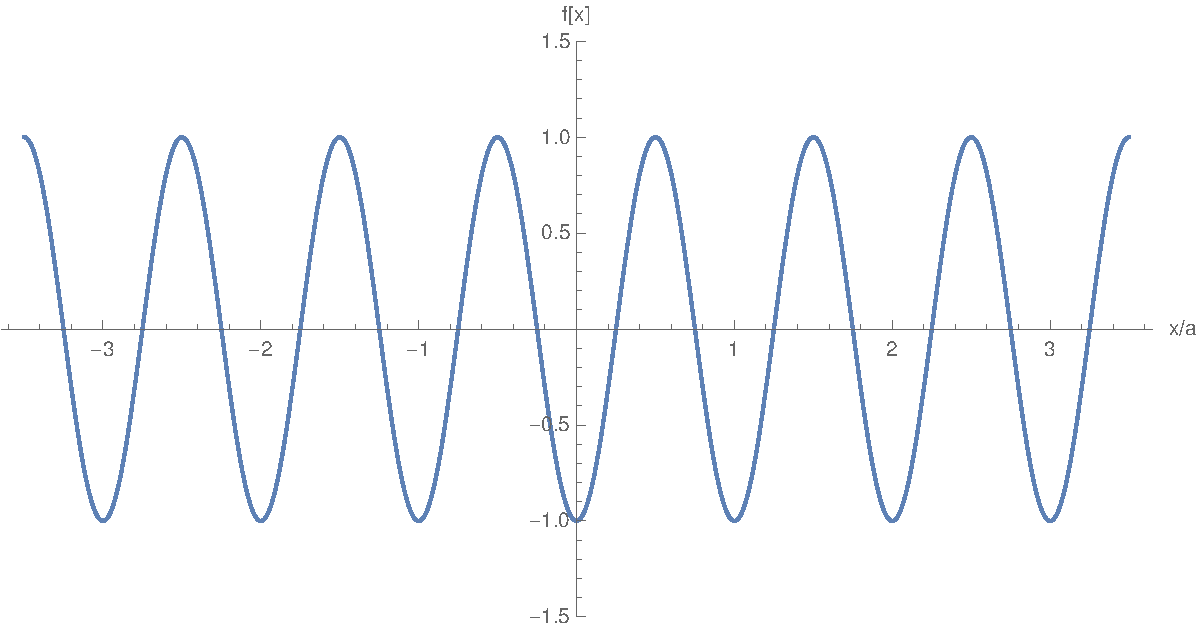
\includegraphics[width=1.0\textwidth]{intro/images/fPlot}
\end{center}
\end{figure}
In terms of its potential
energy due to other particles like itself, it might experience a hard core repulsion with an 
intermediate-range attraction/repulsion, such as the Lennard-Jones 
potential~\cite{atkins2011} shown in 
\begin{figure} \caption[The kind of interaction potential that might exist between two nearby particles.]{The kind of interaction potential that might exist between two nearby particles, $g(x)$. Here we have 
used a Lennard-Jones potential~\cite{atkins2011}, with parameters chosen so that the interaction scale is comparable to the
lattice spacing $a$. The particle generating this potential is located at the origin.} 
\label{fig:partInteraction}
\begin{center}
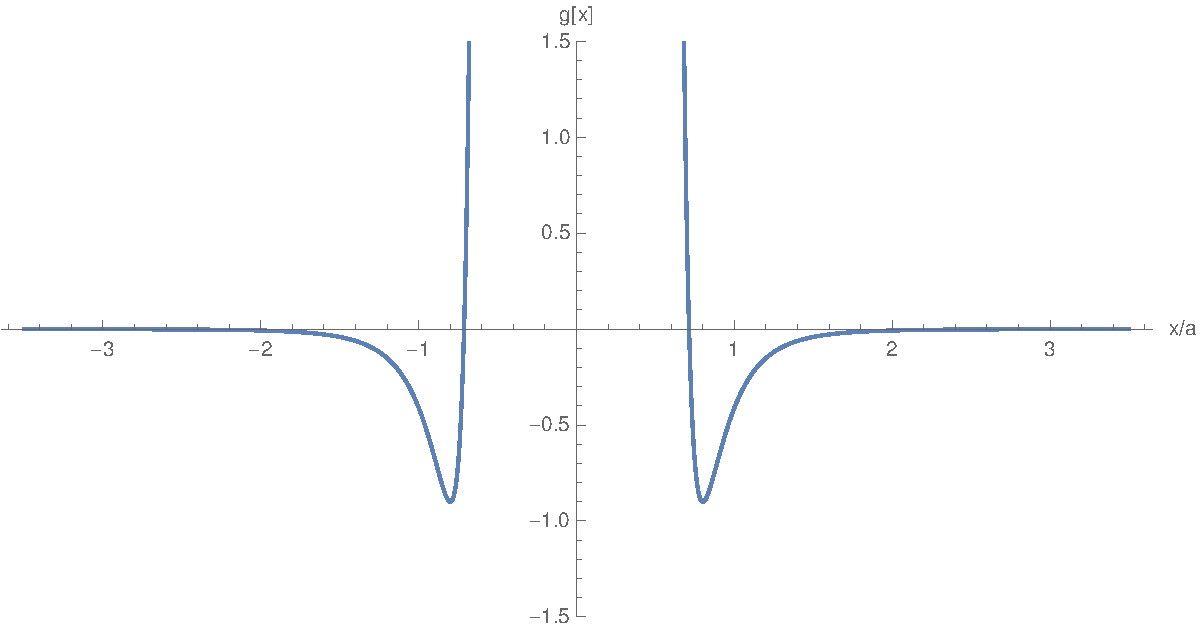
\includegraphics[width=1.0\textwidth]{intro/images/gPlot}
\end{center}
\end{figure}
Fig.~\ref{fig:partInteraction}. Thus, the 
total potential energy landscape from the particle's perspective might look something like 
Fig.~\ref{fig:fullPot}.
\begin{figure} \caption[The sum of the background and interaction potentials.]{The sum of the background
and interaction potentials, the interaction being generated by a particle at the origin. Notice that
the minimum closest to the origin has been greatly deepened, disproportionately to the lowering
of the peak between it and the next-nearest neighbour.} 
\label{fig:fullPot}
\begin{center}
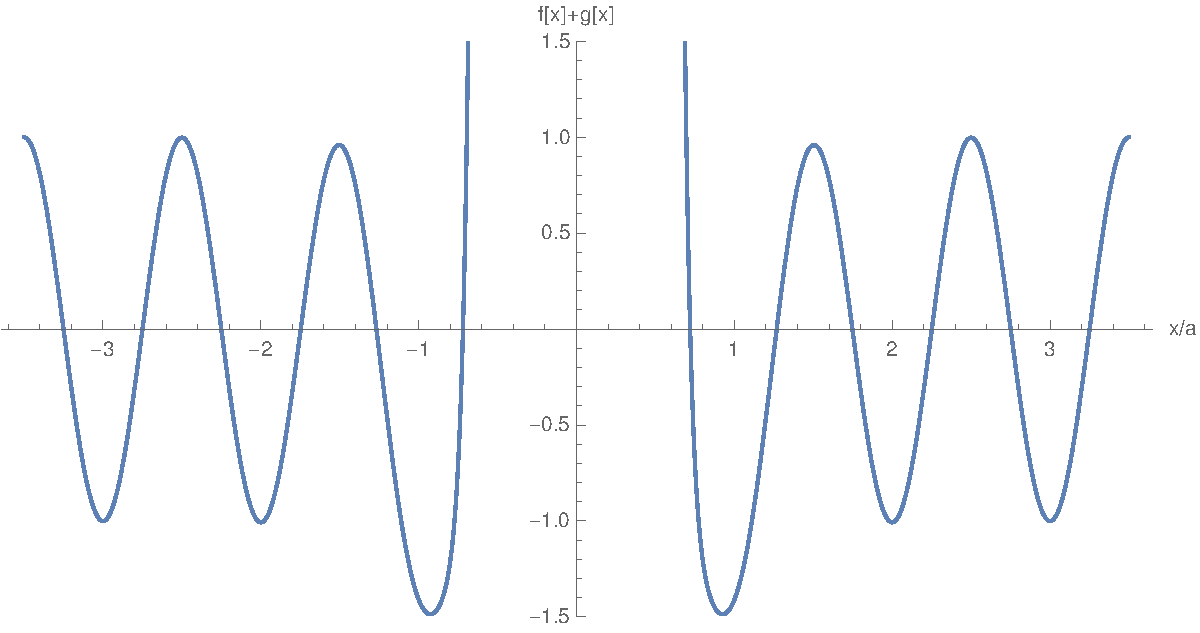
\includegraphics[width=1.0\textwidth]{intro/images/fgSumPlot}
\end{center}
\end{figure}
There are a few things to note here in terms of such a particle moving with
the influence of fluctuating forces:
\begin{enumerate}
\item Particles should be expected to spend the vast majority of their time in the minima of the 
externally-induced potential. This essentially creates a lattice of distinct slots within which a
particle
is highly likely to be at any given time. Thus it is reasonable to speak of particles occupying these 
``slots'' and occasionally transitioning between them.
 \item There is a large potential barrier opposing attempts by particles to get close together. Therefore,
 it is unlikely that multiple particles would be able to squeeze into the same slot,
 and so the assumption that each slot can contain at most one particle is a reasonable one.
 \item If the transition rates between adjacent slots behave in an Arrhenius-like manner~\cite{arrhenius1889, levine2005}, i.e.
 \begin{equation}
  \tau_0^{-1} \propto e^{\frac{\Delta U}{k_B T}},
 \end{equation}
 with $k_B T$ being the characteristic thermal energy,
then the rate of transition is dominated by $\Delta U$, the size of the ``energy barrier'' which
our particle must cross in order to escape from its slot and move to the next one. If we have a relatively
short-ranged intermediate component to the interparticle potential, we can see from Fig.~\ref{fig:fullPot}
that the dominant effect is on the depth of the potential well in which an adjacent particle sits, followed
by the height of the barrier the adjacent particle must cross in order to move away. As these
quantities are altered by different amounts on account of their different distances away from the particle
at the origin, we might expect that \textbf{the dominant affect of the presence of the original particle is
to alter the rate at which an adjacent particle will move away from it}. Of course, the depths and barrier
heights of other slots further away would also in general be affected, but if the interparticle interaction potential decays very rapidly over the length of a lattice spacing these next-neighbour effects will be
very small compared to the nearest-neighbour effect.
\item The particle and background lattice is also assumed to thermalize
after the hop. There 
should be no time-correlated "double hop" events or "two particle"
simultaneous hops.
\end{enumerate}

\subsection{The Sticky Particle Model}
Combining these ideas, we would do well to investigate models that exhibit exclusion (i.e. no more than one 
particle per slot), and in which particles hop away from adjacent particles 
differently to when they are on their 
own. Therefore, we propose a continuous-time Markov process with transition rates as indicated in
Fig.~\ref{fig:transRates}, which we call the Sticky Particle Model (SPM).
\begin{figure} \caption[The transition rates in the Sticky Particle Model.]{The transition rates in the Sticky Particle Model. Here white circles are particles, and black circles are vacancies. Dots indicate connections to the rest of 
the system; the configuration of the particles and vacancies there is irrelevant to the transition here due to the
interaction's short range. Arrows with accompanying quantities indicate possible transitions and their rates, here 
divided by the base rate $\tau_0^{-1}$.} 
\label{fig:transRates}
\begin{center}
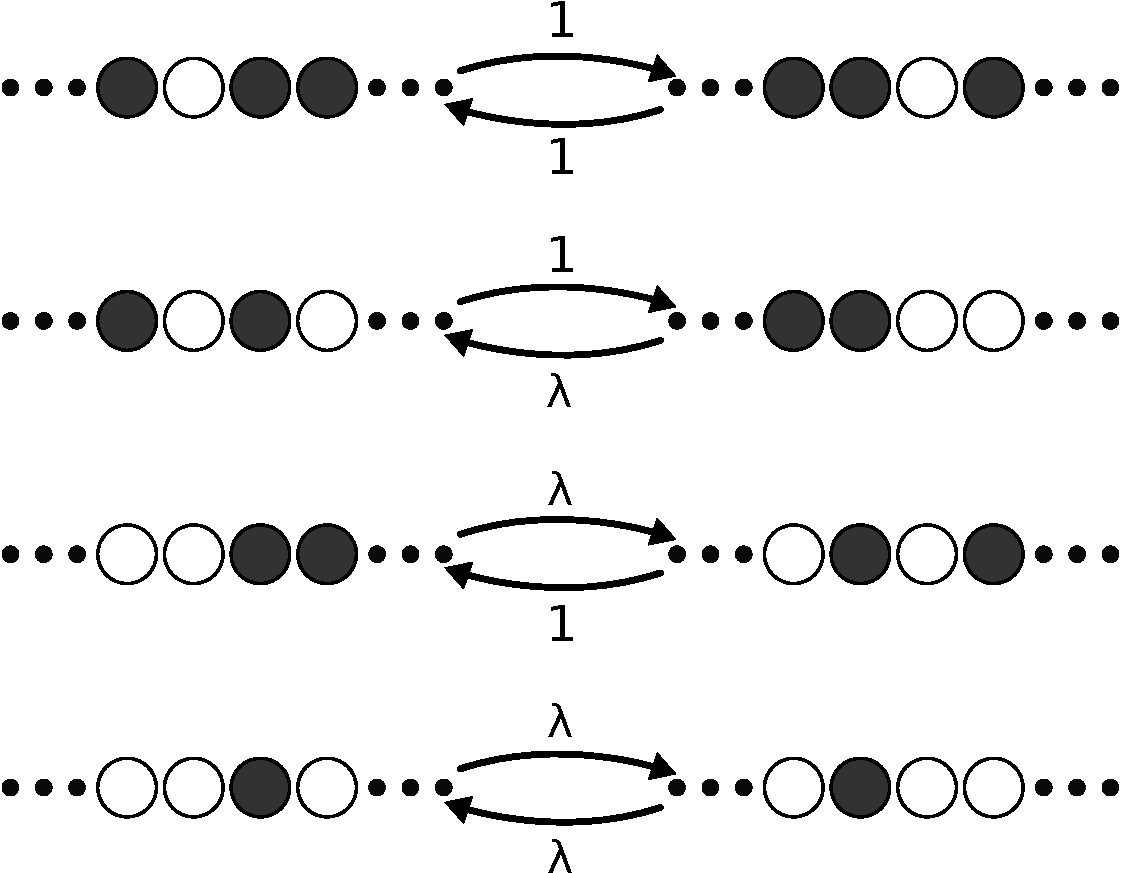
\includegraphics[width=1.0\textwidth]{intro/images/ratesDB}
\end{center}
\end{figure}
A simple verbal description of the model is as follows: particles move randomly into empty adjacent sites with rate 
$\tau_0^{-1}$, unless they are already adjacent to a particle, in which case they jump away from that adjacent
particle with rate $\lambda \tau_0^{-1}$. We have factored out $\tau_0$ because it is the ratio of these two rates,
$\lambda$, that is most important to the phenomenology of this model; rescaling $\tau_0$ is equivalent to 
rescaling time, which is in some sense trivial, whereas varying $\lambda$ should yield models with different behaviours.

Of course, this model is the epitome of a ``toy model'', and with good reason. The complexity of the
analysis of physical models generally scales quite unfavourably with the number of parameters; this model
has the benefit of having only one meaningful parameter, which should make it much easier for us
to explore model behaviour when we use numerical methods.

\section{Properties of the Sticky Particle Model} \label{sec:spmProperties}
Here we list a few properties that the SPM possesses. Note that these properties, although simple, are
often not shared by other models, and in some sense they mark the SPM out by its having all of them.
\subsection{Homogeneity}
The same transition rules apply to any particle in an SPM system regardless of spatial location.
We will break true homogeneity later on when we consider adding boundary conditions, but even then
we still have homogeneous dynamics in the bulk.
\subsection{Symmetry}
One of the more simple aspects of the SPM is its obvious mirror symmetry: that is, the system dynamics
are unchanged by a mirror symmetry transformation. This differentiates it from ASEP-like models~\cite{golinelli2006}; we
will say more about those in Sec.~\ref{sec:asep}. We will refer to this property as \textit{symmetry}.
\subsection{Locality}
The SPM has the property that a particle's transition rates are determined solely by its immediate
environment, in the sense that it can only hop into a space which is empty, and its rate of doing so
then only depends upon what is behind it. By taking account of what is behind it, the model is differentiated from SEP; by not accounting 
for anything further afield, it is not the
same as a more transparently energy-based model might be (although we will see that this model does
have an energy interpretation in Sec.~\ref{sec:dbProof}). We will henceforth refer to this property
as \textit{locality}.
\subsection{Detailed Balance} \label{sec:dbProof}
The SPM possesses the properties of homogeneity, symmetry and locality essentially by design. Indeed, it is
the only exclusion model in $1$D which possesses all of these
properties~\footnote{SEP also obeys these properties, but it is of course 
simply the $\lambda=1$ case of the SPM.}: a particle can only move into
an empty space (exclusion), and so then by locality we need only concern ourselves with its immediate 
neighbours to determine the hopping rate; then there are only two options, depending upon what is in the 
slot the particle is hopping away from, meaning that there are two possible rates, one for each occupation
of that neighbour. But by symmetry and homogeneity, these two rates must apply at every site, and equally
in both directions; thus, adopting all these properties gives us no choice but the SPM.

These rates also imply an additional property. Recall the definition of 
\textbf{detailed balance}~\cite{gardiner1985}:
that there exists
a probability distribution $P$ over configurations $\xi \in \Xi$ such that 
$\forall \xi_1 , \xi_2 \in \Xi $,
  \begin{equation} \label{eq:dbDefn}
    P(\xi_1) \cdot \sigma(\xi_1 \rightarrow \xi_2) = P(\xi_2) \cdot \sigma(\xi_2 \rightarrow \xi_1).
  \end{equation}  
Here, $\Xi$ is the space of all possible configurations for the SPM, and 
$\sigma(a \rightarrow b)$ is the transition rate from state $a$ to state $b$. In our case a transition
means performing one of the operations shown in Fig.~\ref{fig:transRates}. There,
we
list all of the motions that can occur, with all possible local environments: the central two slots must
contain exactly one particle and one vacancy in order for a transition to be possible, and there are two
ways to do this; then there are the two remaining slots at the sides, which can have any of the two
occupations each, so there are $8$ meaningfully different transitions in total.

Consider a probability distribution of the form $P(\xi) \propto \lambda^{-n}$, where $n$ is the total
number of particle-particle adjacencies in the system. In the outer two diagrams of 
Fig.~\ref{fig:transRates}, the forward and backward transition rates are identical, as are the number of
particle-particle adjacencies; thus Eq.~\eqref{eq:dbDefn} is trivially satisfied using the proposed 
distribution $P$. In the middle two diagrams, we see that reducing the number of adjacencies by one
occurs with rate $\lambda$, whilst increasing that number by one happens with rate $1$. Thus, in the 
language of Eq.~\eqref{eq:dbDefn},
\begin{equation}
 \lambda P_0 \cdot 1 = P_0 \cdot \lambda,
\end{equation}
where $P_0$ is a normalisation constant for the probability distribution. We see therefore that the SPM
transition rates satisfy the detailed balance condition with distribution $P$; we can interpret the 
detailed-balance energy as being located in the ``bond'' between two adjacent particles. In hindsight,
that the model obeys detailed balance is perhaps not so surprising; however, it is not immediately 
obvious from the transition rates alone.

An alert reader will have noticed that we still haven't discussed the domain on which the process takes 
place very much. In our detailed balance proof we used only the SPM bulk rates, 
so that this result only
applies to SPM systems defined on an infinite domain or on a finite ring. If one introduces boundaries,
and defines additional rates to define their behaviour, one will typically end up breaking detailed 
balance.

\section{Relationship to Existing Models} \label{sec:existingModels}
Of course, the SPM is not exactly ``new'': it is very similar to several models already discussed in the
literature. Here we will discuss the more prominent of these, with emphasis on why the SPM is different or
how we are going to analyse it differently to them.
\subsection{The Ising Model}
The SPM is equivalent to a constrained version of the classical Ising 
model~\cite{lenz1920, Ising1925, strecka2015} in $1$D; we can map SPM
occupations $\rho_i \in {0, 1}$ on to Ising spins $\sigma_i \in {-1, 1}$ via the transformation
\begin{equation}
 \sigma_i = 2 \rho_i - 1 .
\end{equation}
The constraint is that the magnetisation is locally conserved, i.e. we can only swap the spins of adjacent
sites during the dynamics. If we are careful with our definitions of the SPM transition rates,
the SPM is a equivalent to a method for numerically simulating the Ising model known as Kawasaki
dynamics, which has been in the literature for a long time~\cite{kawasaki1966, Garrido1990, grynberg2010}. 
Kawasaki dynamics was originally intended as
a stochastic Markov process designed to replicate the Ising model in equilibrium, albeit with a
constraint on the magnetisation, which makes more sense when the
dynamics are interpreted as a model of a two-species alloy. We have more 
to say about the correspondence with the Ising model in Sec.~\ref{sec:isingSim}.

In theory, one can calculate equilibrium properties of the SPM by using this equivalence to the constrained
Ising model; in order to do this, one may attempt to implement the constraint by varying the applied
magnetic field in such a way that the system ends up with the correct magnetisation, and then working
out desired quantities from there using the Ising partition function~\cite{baxter2016}. However, we found that
this results
in extremely convoluted algebra, and it is actually easier to build a new partition for the SPM from 
scratch, as we have done in Sec.~\ref{sec:spmPartFn}.
\subsection{SEP/ASEP/TASEP} \label{sec:asep}
The SPM also resembles the SEP/ASEP/TASEP family of models~\cite{liggett1985, golinelli2006, blythe2007,
Crampe2014}, 
as it is an
exclusion process. However, we 
have not found this resemblance to be particularly helpful, as these models do not contain the
nearest-neighbour interactions between particles that the SPM does. Thus, we do not believe that we are
able to solve the SPM using a similar matrix product solution to TASEP. Furthermore, ASEP and TASEP
are manifestly asymmetric in their bulk dynamics, whereas the SPM is not.

\subsection{The KLS Model}
The Katz-Lebowitz-Spohn (KLS) model~\cite{Katz1984, Zia2010} was originally designed to model the
behaviour of ions moving stochastically
under the influence of an external potential. The SPM is in fact a specific symmetric case of the
$1$-dimensional KLS model. Whilst the KLS model exhibits plenty of interesting behaviour
(in particular, the formation of stripes during flow in higher dimensions), most of the research done
into it has involved using asymmetric versions of the model to drive flow. The stationary
distribution for the symmetric version on a ring is given in~\cite{Katz1984}, whilst the version with open boundaries
which we study here has received far less attention.

\section{Research Outline}
Our investigation into the SPM has focussed primarily upon its flow characteristics when driven
by concentration gradients imposed by boundary conditions. This does not seem to have been something
which has been investigated much before; as we have hinted in Sec.~\ref{sec:existingModels}, most
research into flow in many-body systems uses internal dynamics to drive the flow instead of the 
boundaries. Therefore, we are essentially working from scratch with this model.
To present our results, we are using the following structure:
\begin{itemize}
 \item We use primarily analytic methods in Ch.~\ref{sec:analChap}. These include the evaluation
 of the partition function for the SPM on a closed ring (Sec.~\ref{sec:spmPartFn}), the development
 of the mean-field theory of the SPM (Sec.~\ref{sec:spmMft}) and its generalisation to higher dimensions
 (Sec.~\ref{sec:highDimSPM}).
 \item In Ch.~\ref{sec:transRateChapter} we introduce a method for using sparse numerical linear
 algebra to exactly solve the steady state distribution for small $1$D SPM systems. We also show how this
 method can be used to compute some time-dependent quantities in Sec.~\ref{sec:TRMTimeDep}.
 \item In Ch.~\ref{sec:numerics} we discuss the use of Monte-Carlo methods to calculate the properties
 of the SPM in somewhat larger $1$D and $2$D systems. In particular we focus on the Kinetic
  Monte-Carlo algorithm (KMC) in Sec.~\ref{sec:nFoldWay}, and calculate the bulk of our results
  using it.
\item We summarise our main conclusions in Ch.~\ref{sec:conclusionsChap}.
\end{itemize}


% mention Ising and ASEP
